%%%%%%%%%%%%%%%%%%%%%%%%%%%%%%%%%%%%%%%%%
% Dreuw & Deselaer's Poster
% LaTeX Template
% Version 1.0 (11/04/13)
%
% Created by:
% Philippe Dreuw and Thomas Deselaers
% http://www-i6.informatik.rwth-aachen.de/~dreuw/latexbeamerposter.php
%
% This template has been downloaded from:
% http://www.LaTeXTemplates.com
%
% License:
% CC BY-NC-SA 3.0 (http://creativecommons.org/licenses/by-nc-sa/3.0/)
%
%%%%%%%%%%%%%%%%%%%%%%%%%%%%%%%%%%%%%%%%%

%----------------------------------------------------------------------------------------
%	PACKAGES AND OTHER DOCUMENT CONFIGURATIONS
%----------------------------------------------------------------------------------------

\documentclass[final,hyperref={pdfpagelabels=false}]{beamer}

\usepackage[orientation=portrait,size=a0,scale=1.4]{beamerposter} % Use the beamerposter package for laying out the poster with a portrait orientation and an a0 paper size

\usetheme{I6pd2} % Use the I6pd2 theme supplied with this template

\usepackage[english]{babel} % English language/hyphenation

\usepackage{amsmath,amsthm,amssymb,latexsym} % For including math equations, theorems, symbols, etc

%\usepackage{times}\usefonttheme{professionalfonts}  % Uncomment to use Times as the main font
%\usefonttheme[onlymath]{serif} % Uncomment to use a Serif font within math environments

\boldmath % Use bold for everything within the math environment

\usepackage{booktabs} % Top and bottom rules for tables

\graphicspath{{figures/}} % Location of the graphics files

\usecaptiontemplate{\small\structure{\insertcaptionname~\insertcaptionnumber: }\insertcaption} % A fix for figure numbering

%----------------------------------------------------------------------------------------
%	TITLE SECTION 
%----------------------------------------------------------------------------------------

\title{\huge  ~\vspace{10mm} \newline  Multi Data Source Stock Market Prediction} 


\author{\huge~\vspace{10mm} \newline  Yuhan Su, Ruichuang Cao, Wei Xu} % Author(s)


\institute{\huge Tsinghua University} % Institution(s)

%----------------------------------------------------------------------------------------
%	FOOTER TEXT
%----------------------------------------------------------------------------------------

\newcommand{\leftfoot}{Tsinghua University. http://iiis.tsinghua.edu.cn} % Left footer text

\newcommand{\rightfoot}{IBM SuperVessel Cloud. https://ptopenlab.com} % Right footer text

%----------------------------------------------------------------------------------------

\begin{document}
\linespread{0.98}	
\addtobeamertemplate{block end}{}{\vspace*{3ex}} % White space under blocks

\begin{frame}[t] % The whole poster is enclosed in one beamer frame

\begin{columns}[t] % The whole poster consists of two major columns, each of which can be subdivided further with another \begin{columns} block - the [t] argument aligns each column's content to the top

\begin{column}{.03\textwidth}\end{column} % Empty spacer column

\begin{column}{.445\textwidth} % The first column

%----------------------------------------------------------------------------------------
%	INTRODUCTION
%----------------------------------------------------------------------------------------

\begin{block}{Introduction}
\begin{itemize}	
\item Everyone dreams to predict stock price changes. Some even succeeded -- to some degree. 
\item China stock market is influenced by rumors on social media.
\end{itemize}
\centering
\begin{figure}
	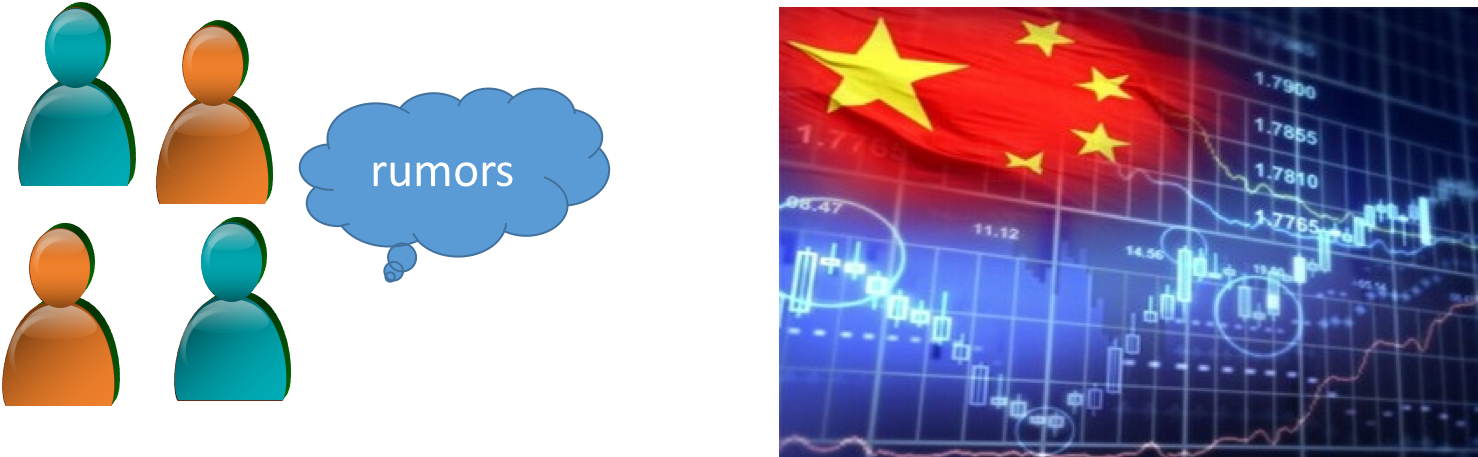
\includegraphics[width=0.6\linewidth]{intro.png}
	%\caption{Rumors in stock market}
	\label{intro}
\end{figure}
\begin{itemize}
\item We build a real-time data stream stock prediction system on IBM SuperVessel Cloud.  
\item We can use multiple data sources, including trading data and social media rumors. 

\end{itemize}
\end{block}

%----------------------------------------------------------------------------------------
%	OBJECTIVES
%----------------------------------------------------------------------------------------

\begin{block}{Contribution}

\begin{itemize}
\item A system to process real-time data stream from multiple sources. 
\item Use multi data source, including trading data and social rumors, to predict stock market in China.
\item A scalable system using the state-of-the-art cloud technology. 
\item An intuitive web UI to let users edit and analyze code and data.
\end{itemize}
\centering
\begin{figure}
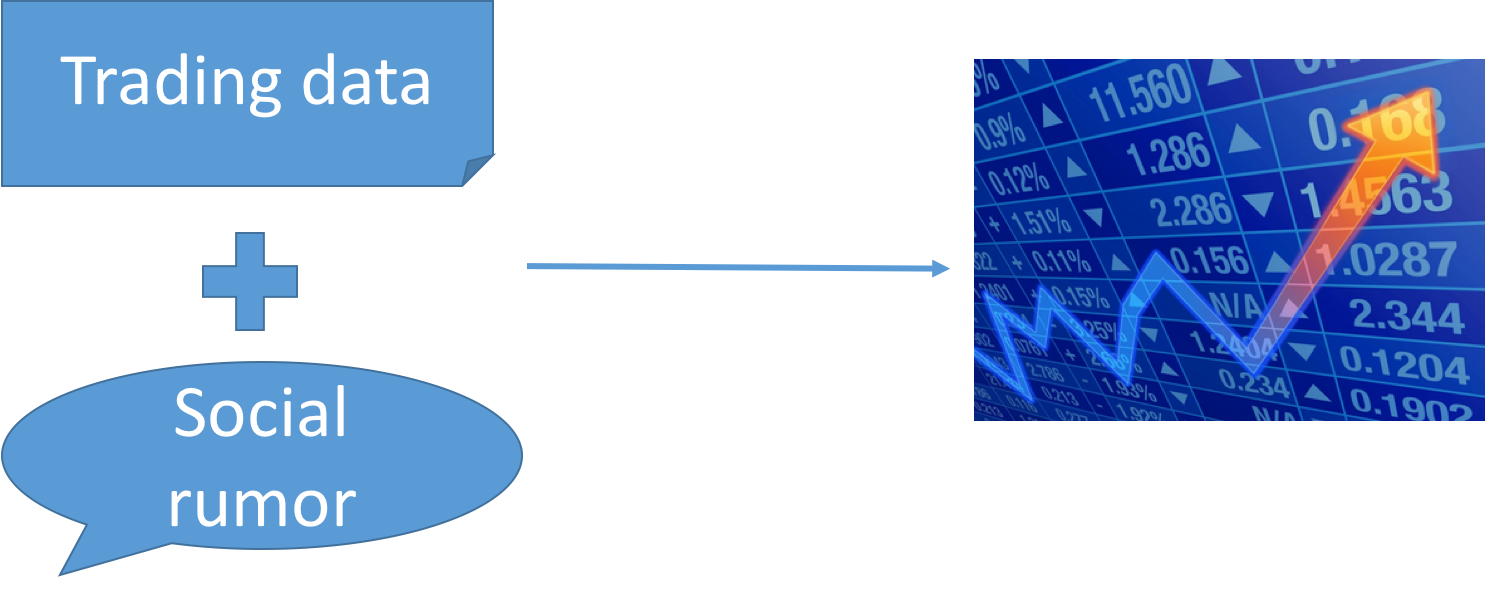
\includegraphics[width=0.5\linewidth]{intuition.png}
%\caption{Data for prediction}
\label{sample}
\end{figure}

\end{block}

%----------------------------------------------------------------------------------------
%	MATERIALS
%----------------------------------------------------------------------------------------

\begin{block}{Data Source}

%\begin{columns} % Subdivide the first main column

%\begin{column}{.56\textwidth} % The first subdivided column within the first main column

\begin{itemize}
\item SSE50 index history. Daily closing price. Also our predicting target.
\item Sina Stock Forum. Posts and comments from http://guba.sina.com.cn.

%\end{column}

%\begin{column}{.4\textwidth} % The second subdivided column within the first main column

%\end{column}
%\end{columns} % End of the subdivision

\item Financial news. Collected from Tushare.
\item NASQAF index. Daily closing price.
\item RMB Exchange rate. Daily value.
\end{itemize}

\centering
\begin{figure}

\includegraphics[width=1.0\linewidth]{datasource.png}
%\caption{Multi data source}
\label{sample}
\end{figure}

\end{block}


\begin{block}{Data Pre-Processing}

\begin{itemize}
\item Leveraging the cloud to do multi-step data pre-processing as streams. 

\item Rumors and news $\rightarrow$ sentiment (left figure)

\item Trading history $\rightarrow$ values within a certain window (right figure)

\begin{columns} % Subdivide the first main column
\begin{column}{.4\textwidth} 
	\begin{figure}
		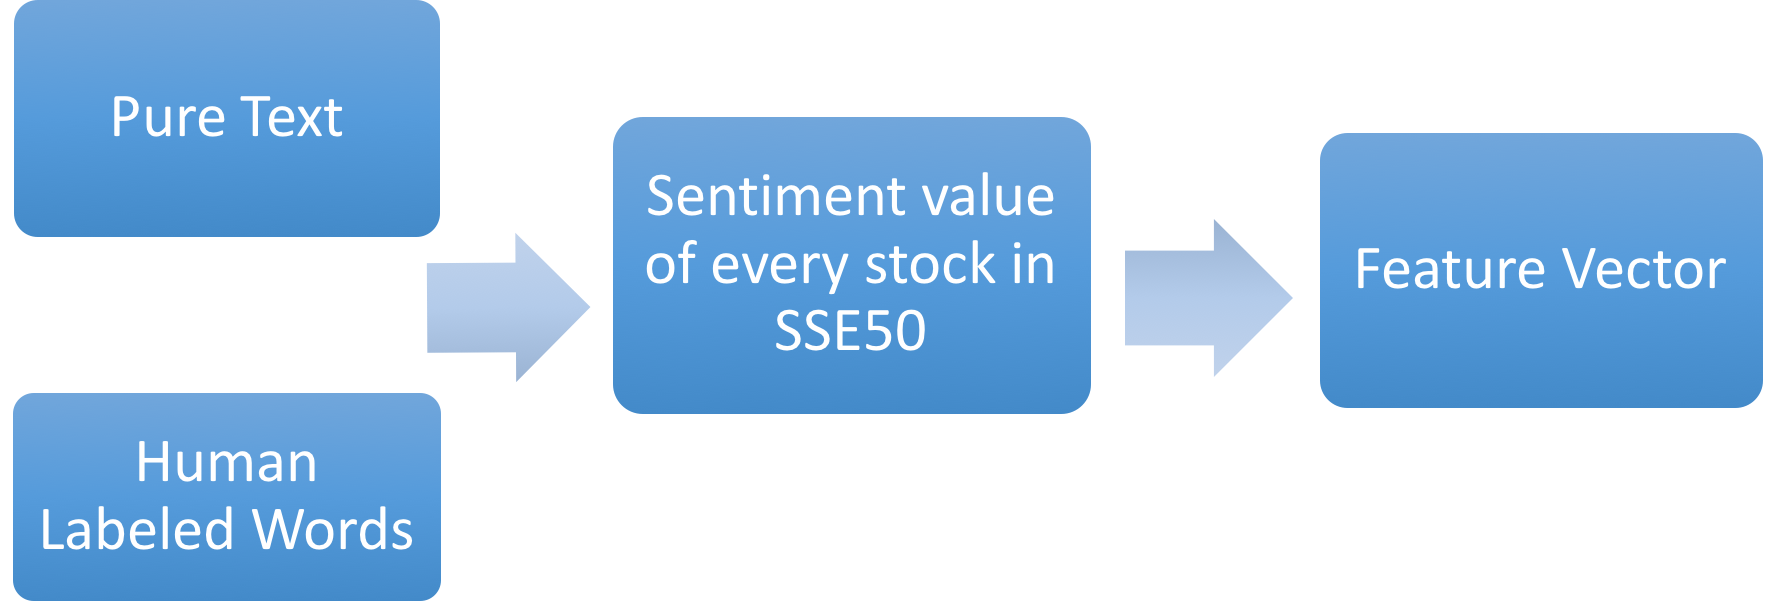
\includegraphics[width=1.2\linewidth]{textdata.png}
		%\caption{Rumors/News data}
		\label{text}
	\end{figure}
\end{column}
\begin{column}{.4\textwidth} 
	\begin{figure}
		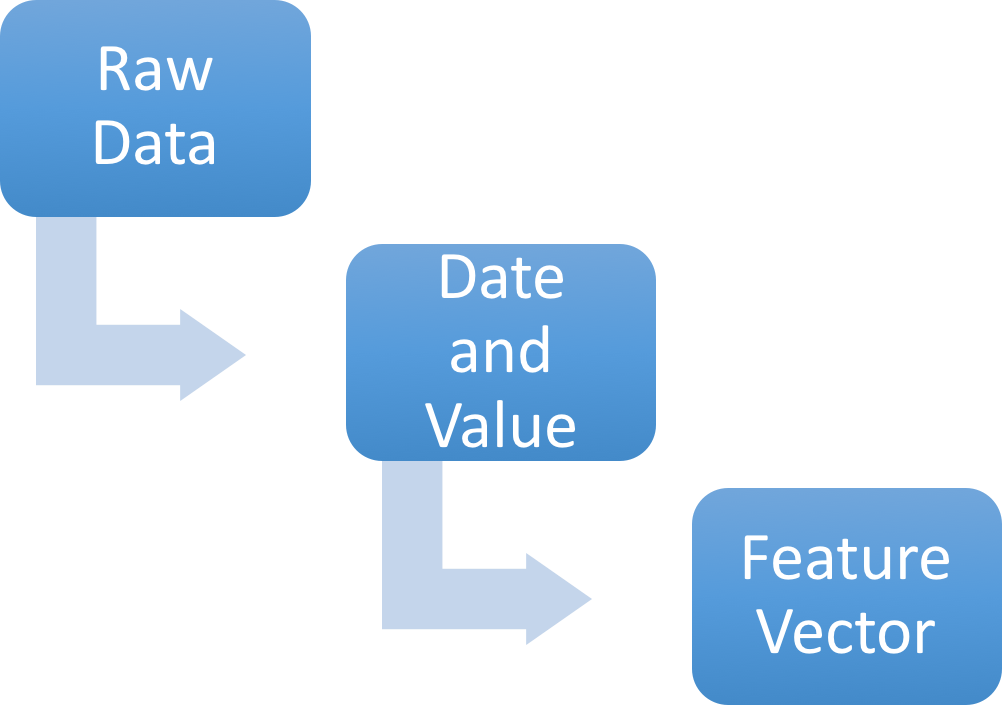
\includegraphics[width=0.8\linewidth]{numdata.png}
		%\caption{Trading history data}
		\label{num}
	\end{figure}
\end{column}
\end{columns}

\end{itemize}
\end{block}


\end{column} % End of the first column

\begin{column}{.02\textwidth}\end{column} % Empty spacer column

\begin{column}{.445\textwidth} % The second column

%----------------------------------------------------------------------------------------
%	METHODS
%----------------------------------------------------------------------------------------

%----------------------------------------------------------------------------------------


%------------------------------------------------

\begin{block}{System Architecture}
	\begin{figure}
		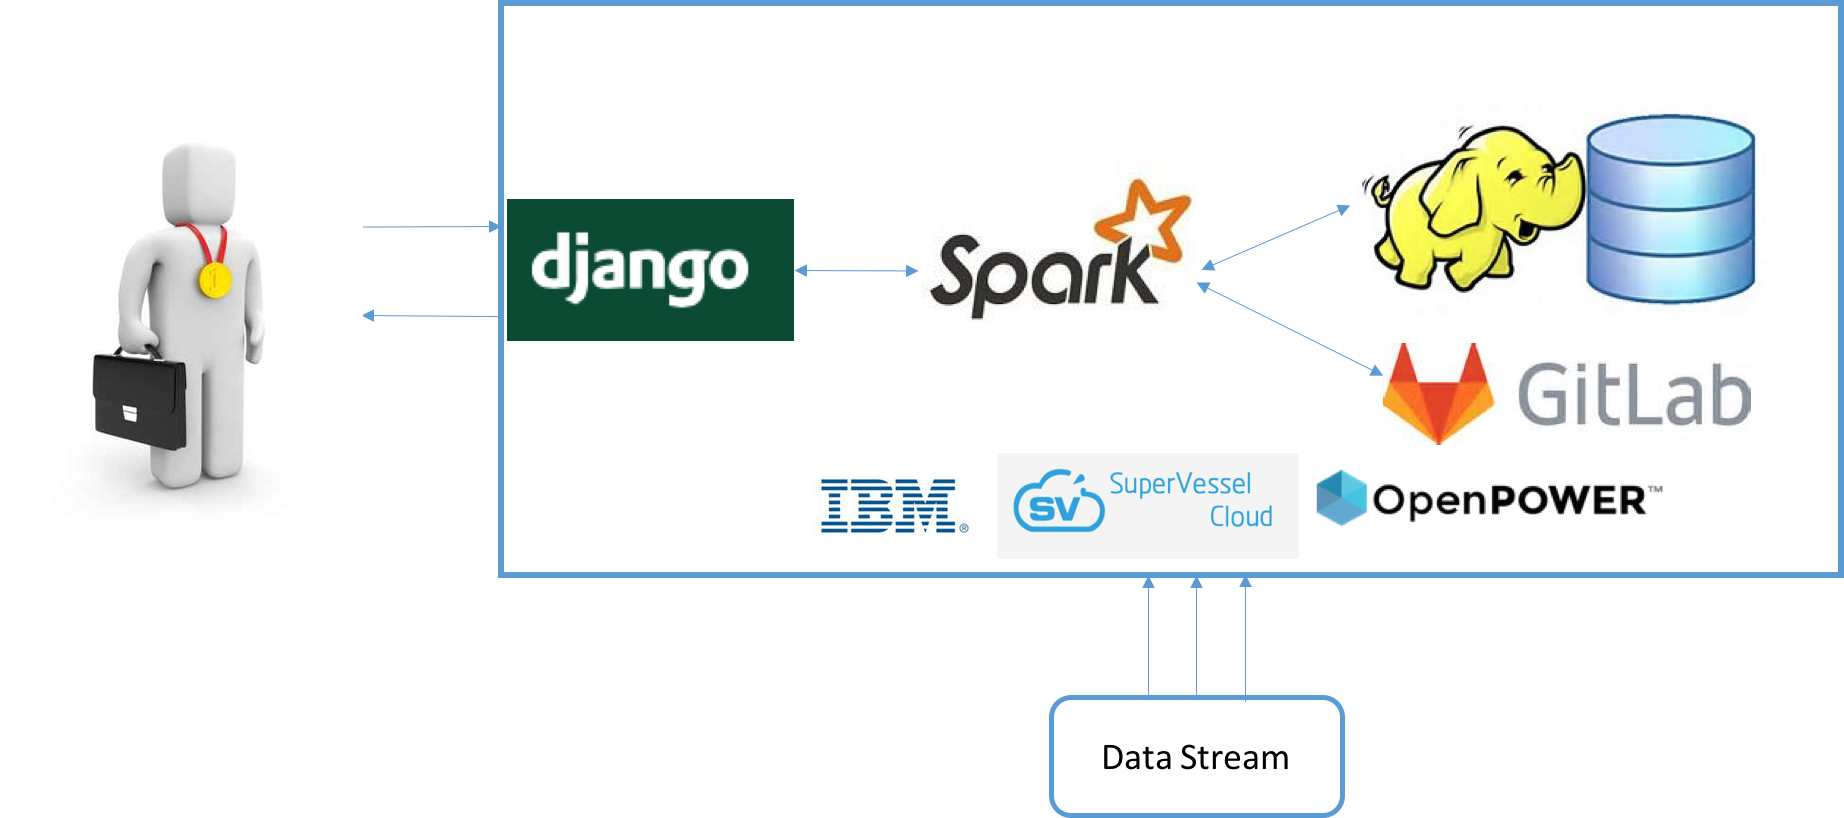
\includegraphics[width=0.7\linewidth]{system.png}
		%\caption{System Architecture}
	\end{figure}
\begin{itemize}
\item Building blocks: Spark, HDFS, Gitlab, Django
\item They all run efficiently on IBM SuperVessel Cloud. 
\item Integrates the acquisition, preprocessing and learning of data source streams, and shows the final prediction result. 
\item Everything under a single web UI. Users can change the model parameters, modify the codes, and check the running status online.

\end{itemize}

\begin{figure}
		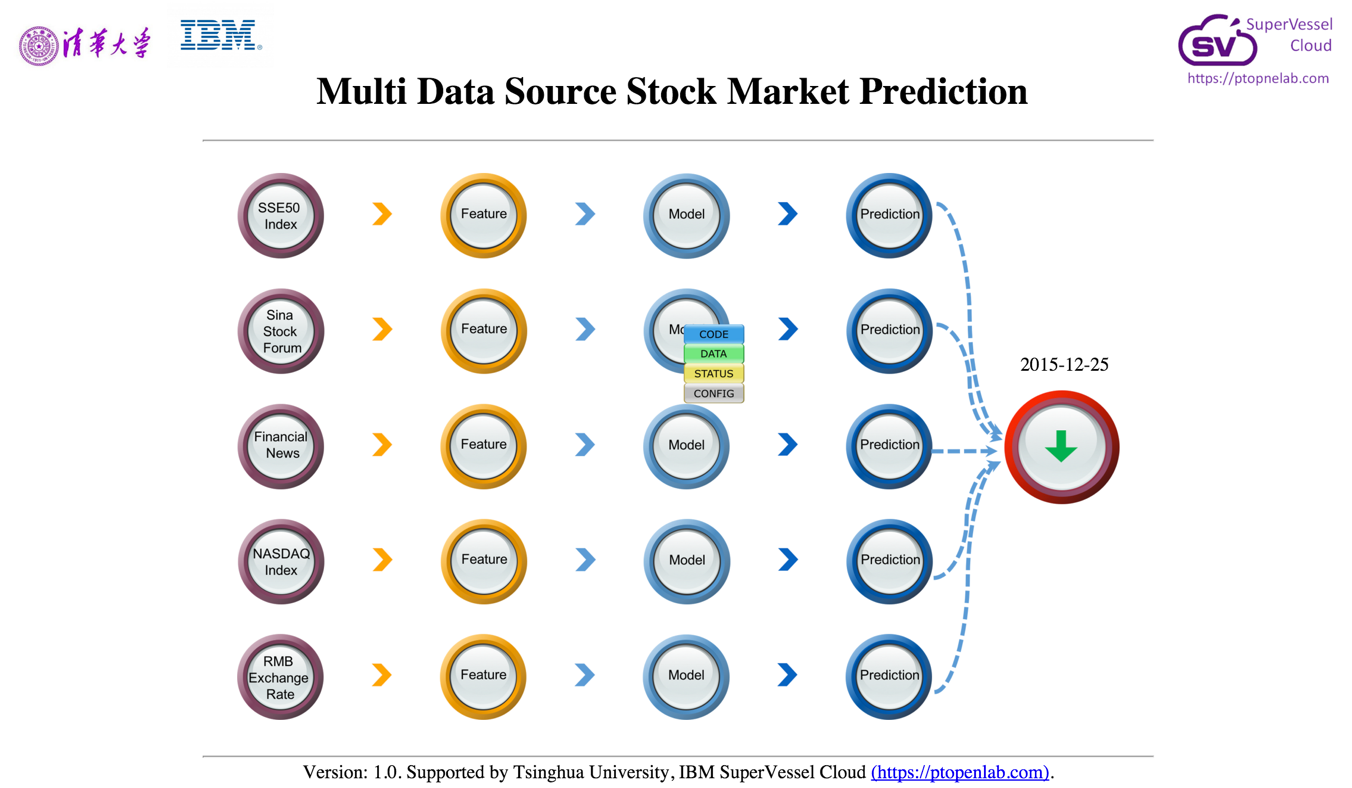
\includegraphics[width=0.5\linewidth]{webui.png}
		%\caption{Web UI}
	\end{figure}

\end{block}

\begin{block}{SuperVessel Cloud}
\begin{columns} % Subdivide the first main column
\begin{column}{.3\textwidth} 
	\begin{figure}
		
\includegraphics[width=0.7\linewidth]{ibm.png}
		%\caption{SuperVessel Cloud}
		\label{sv}
	\end{figure}
\end{column}
\begin{column}{.3\textwidth} 
	\begin{figure}
		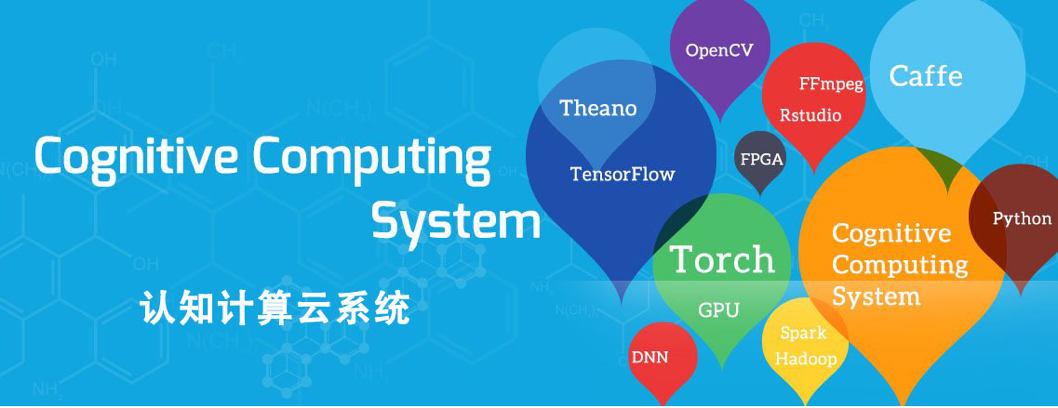
\includegraphics[width=1.0\linewidth]{svcloud.png}
		%\caption{SuperVessel Cloud}
		\label{sv}
	\end{figure}
\end{column}
\begin{column}{.3\textwidth} 
	\begin{figure}
		
\includegraphics[width=0.7\linewidth]{svlogo.png}
		%\caption{SuperVessel Cloud}
		\label{svl}
	\end{figure}
\end{column}
\end{columns}

\begin{itemize}
\item We use SuperVessel Cloud, based on OpenPOWER technology and provides the high efficiency cognitive computing infrastructure for frontier science with high performance heterogenous platform (GPU/FPGA).

\item SuperVessel provides three handy services: basic cognitive cloud service, cognitive computing service platform, and application acceleration store for new technology sharing. 

\item SuperVessel provides us with a scalable and easy-to-maintain cloud infrastructure to build our systems on. 
\end{itemize}



 \begin{figure}
		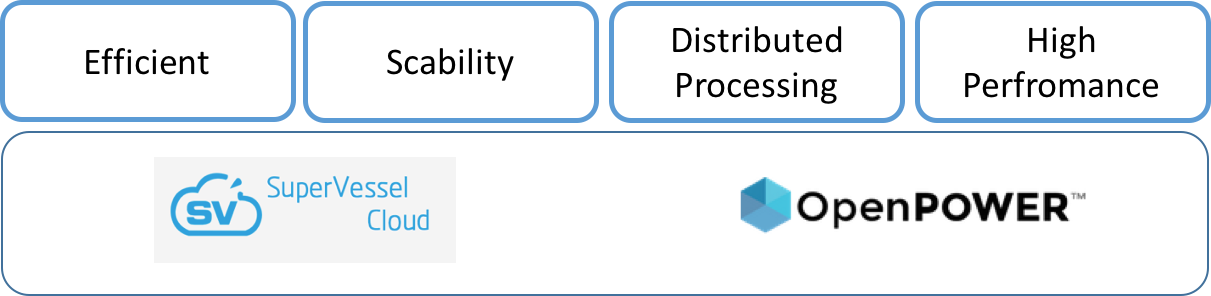
\includegraphics[width=0.7\linewidth]{openpower.png}
		%\caption{System Architecture}
	\end{figure}
\end{block}

%----------------------------------------------------------------------------------------
%	CONCLUSION
%----------------------------------------------------------------------------------------

\begin{block}{Conclusion}

\begin{itemize}
\item Using multiple data sources improves stock prediction. 
\item We can provide the entire analysis under an intuitive web UI.
\item Highly efficient cognitive computing infrastructure at SuperVessel greatly simplified our development.
\end{itemize}

\end{block}

%----------------------------------------------------------------------------------------
%	ACKNOWLEDGEMENTS
%----------------------------------------------------------------------------------------

\begin{block}{Acknowledgments}

\begin{itemize}
\item IBM China Research Lab provided the SuperVessel Cloud. 
\item IBM partly funded this project.
\item Tushare website provided datasets. 
\end{itemize}

\end{block}

%----------------------------------------------------------------------------------------
%	CONTACT INFORMATION
%----------------------------------------------------------------------------------------

\setbeamercolor{block title}{fg=black,bg=orange!70} % Change the block title color

\begin{block}{Contact Information}

\begin{itemize}
\item Web: http://iiis.tsinghua.edu.cn ~~ https://ptopenlab.com \\


\item Email: Yuhan Su~~~~~~~~~~\href{mailto:syhmartin@yeah.ne}{syhmartin@yeah.net} \\ 
~~~~~~~~~~Ruichuang Cao~~\href{mailto:create0818@163.com}{create0818@163.com} \\
~~~~~~~~~~Prof. Wei Xu~~~~~~\href{mailto:wei.xu.0@gmail.com}{wei.xu.0@gmail.com}
\end{itemize}

\end{block}

%----------------------------------------------------------------------------------------

\end{column} % End of the second column

\begin{column}{.015\textwidth}\end{column} % Empty spacer column

\end{columns} % End of all the columns in the poster

\end{frame} % End of the enclosing frame
\end{document}